\begin{center}
    \textbf{Superposition of waves}
    \begin{quote}
        \textit{When two or more waves travel in the same medium, they are bound to interact with each other. They retain their wave nature after combining with each other, but usually, the resultant wave is different from both of the individual waves. The superposition principle helps us describe the resulting wave or motion that is produced when two or more waves combine with each other. }
    \end{quote}
\end{center}
\begin{itemize}
    \item Two sin waves with different frequencies but same amplitudes\\
    \begin{tikzpicture}
        \begin{scope}
            \tzaxes(0, -1)(2.25*pi, 1.5){$x$}{$y_2$}
            \tzfn{sin(deg(2*\x))}[0:2*pi]
        \end{scope}
        \begin{scope}[yshift=4cm]
            \tzaxes(0, -1)(2.25*pi, 1.5){$x$}{$y_1$}
            \tzfn{sin(deg(\x))}[0:2*pi]
        \end{scope}
        \tznode(2.5*pi, 2){$\Rightarrow$}
        \begin{scope}[xshift=9cm, yshift=2cm]
            \tzaxes(0, -1)(2.25*pi, 2){$x$}{$y_1+y_2$}
            \tzfn{sin(deg(\x)) + sin(deg(2*\x))}[0:2*pi]
        \end{scope}
    \end{tikzpicture}
    
    \item Two sin waves with same frequencies but different amplitudes\\
    \begin{tikzpicture}
        \begin{scope}
            \tzaxes(0, -1)(2.25*pi, 1.5){$x$}{$y_2$}
            \tzfn{0.5*sin(deg(2*\x))}[0:2*pi]
        \end{scope}
        \begin{scope}[yshift=4cm]
            \tzaxes(0, -1)(2.25*pi, 1.5){$x$}{$y_1$}
            \tzfn{sin(deg(2*\x))}[0:2*pi]
        \end{scope}
        \tznode(2.5*pi, 2){$\Rightarrow$}
        \begin{scope}[xshift=9cm, yshift=2cm]
            \tzaxes(0, -1)(2.25*pi, 2){$x$}{$y_1+y_2$}
            \tzfn{sin(deg(2*\x)) + 0.5*sin(deg(2*\x))}[0:2*pi]
        \end{scope} 
    \end{tikzpicture}

    \item Two sin waves with different frequencies and amplitudes\\
    \begin{tikzpicture}
        \begin{scope}
            \tzaxes(0, -1)(2.25*pi, 1.5){$x$}{$y_2$}
            \tzfn{0.5*sin(deg(2*\x))}[0:2*pi]
        \end{scope}
        \begin{scope}[yshift=4cm]
            \tzaxes(0, -1)(2.25*pi, 1.5){$x$}{$y_1$}
            \tzfn{sin(deg(3*\x))}[0:2*pi]
        \end{scope}
        \tznode(2.5*pi, 2){$\Rightarrow$}
        \begin{scope}[xshift=9cm, yshift=2cm]
            \tzaxes(0, -1)(2.25*pi, 2){$x$}{$y_1+y_2$}
            \tzfn{sin(deg(3*\x)) + 0.5*sin(deg(2*\x))}[0:2*pi]
        \end{scope} 
    \end{tikzpicture}

    \begin{center}
        \begin{quote}
            \textit{In reality, waves are not limited to simple sinusoidal waves. They can be any shape, and the superposition principle applies to all of them.\\[2mm]
            Almost all waves(continuous and differentiable) can be described as a superposition of simpler waves, means that the wave can be broken down into a sum of sinusoidal waves.}
        \end{quote}
        \begin{tikzpicture}
            \begin{scope}
                \tzaxes(0, -1)(2.25*pi, 1.25){$x$}{$y_3$}
                \tzfn{sin(deg(8*\x))}[0:2*pi]
            \end{scope}
            \begin{scope}[yshift=3cm]
                \tzaxes(0, -1)(2.25*pi, 1.25){$x$}{$y_2$}
                \tzfn{sin(deg(4*\x))}[0:2*pi]
            \end{scope}
            \begin{scope}[yshift=6cm]
                \tzaxes(0, -1)(2.25*pi, 1.25){$x$}{$y_1$}
                \tzfn{sin(deg(2*\x))}[0:2*pi]
            \end{scope}
            \tznode(2.5*pi, 3){$\Rightarrow$}
            \begin{scope}[xshift=9cm, yshift=3cm]
                \tzaxes(0, -2)(2.25*pi, 3){$x$}{$y_1+y_2+y_3$}
                \tzfn{sin(deg(2*\x)) + sin(deg(4*\x)) + sin(deg(8*\x))}[0:2*pi]
            \end{scope} 
        \end{tikzpicture}
    \end{center}

    \item \textbf{Resultant Amplitude and Intensity due to two coherent waves}\\
    \textbf{Coherent Waves }: \textit{Two waves are said to be coherent if their frequencies are same. But actually we define coherence of wave according to phase difference, means there should be a constant phase difference for the waves to be coherent.}

    \begin{itemize}
        \item \textbf{resultant amplitude}
        \begin{align*}
            y_1 &= A_1 \sin(kx-\omega t + \phi_1)\\
            y_2 &= A_2 \sin(kx-\omega t + \phi_2)\\
            y &= y_1 + y_2\\
            y &= A_1 \sin(kx-\omega t + \phi_1) + A_2 \sin(kx-\omega t + \phi_2)\\
                &= A_1 \sin(kx-\omega t) \cos(\phi_1) + A_1 \cos(kx-\omega t) \sin(\phi_1) + \\ &\quad A_2 \sin(kx-\omega t) \cos(\phi_2) + A_2 \cos(kx-\omega t) \sin(\phi_2)\\
                &= \sin(kx-\omega t) \underbrace{(A_1 \cos(\phi_1) + A_2 \cos(\phi_2))}_{A\cos(\phi)} + \cos(kx-\omega t) \underbrace{(A_1 \sin(\phi_1) + A_2 \sin(\phi_2))}_{A\sin(\phi)}\\
              \Aboxed{y  &= A \sin(kx-\omega t + \phi)}\\
        \end{align*}
        \begin{align*}
            A\cos(\phi) &= A_1 \cos(\phi_1) + A_2 \cos(\phi_2)\\
            A\sin(\phi) &= A_1 \sin(\phi_1) + A_2 \sin(\phi_2)\\
            \intertext{Squaring and adding both the equations,}
            A^2\cos^2(\phi) + A^2\sin^2(\phi) &= (A_1 \cos(\phi_1) + A_2 \cos(\phi_2))^2 + (A_1 \sin(\phi_1) + A_2 \sin(\phi_2))^2\\
            A^2 &= A_1^2 + A_2^2 + 2A_1A_2(\cos(\phi_1)\cos(\phi_2) + \sin(\phi_1)\sin(\phi_2))\\
            A^2 &= A_1^2 + A_2^2 + 2A_1A_2\cos(\phi_1 - \phi_2)\\
            \Aboxed{A &= \sqrt{A_1^2 + A_2^2 + 2A_1A_2\cos(\phi_1 - \phi_2)}}\\
            \intertext{Also, one more relation we can derive from the above equations,}
            \tan(\phi) &= \frac{A_1 \sin(\phi_1) + A_2 \sin(\phi_2)}{A_1 \cos(\phi_1) + A_2 \cos(\phi_2)}\\
            \Aboxed{\phi &= \tan^{-1}\left(\frac{A_1 \sin(\phi_1) + A_2 \sin(\phi_2)}{A_1 \cos(\phi_1) + A_2 \cos(\phi_2)}\right)}\\
        \end{align*}
        \begin{center}
            \begin{tikzpicture}
                \tzline[->](0, 0)(4, 0){$\vec{A_1}$}[r]
                \tzline[->](0, 0)(2, 3){$\vec{A_2}$}[a]
                \tzline[->](0, 0)(5, 3){$\vec{A}$}[a]
                \tzanglemark(2, 0)(0, 0)(5, 3){$\phi$}(35pt)
                \tzanglemark(4, 0)(0, 0)(2, 3){$\Delta \phi$}(15pt)
                \tznode(2.5, -1){\textit{also we can analyze the resultant amplitude using vector method}}
            \end{tikzpicture}
        \end{center}
        \item \textbf{resultant intensity}
        \begin{align*}
            \intertext{from the equation for intensity,}
            I &= \frac{1}{2} \rho \omega^2 A^2 v\\
            I &\propto A^2\\
            A^2 &= A_1^2 + A_2^2 + 2A_1A_2\cos(\phi_1 - \phi_2)\\
            \Aboxed{I &= I_1 + I_2 + 2\sqrt{I_1I_2}\cos(\phi_1 - \phi_2)}\\
            \intertext{Special case, when $A_1=A_2=A_0$}
            A^2 &= A_0^2 + A_0^2 + 2A_0^2\cos(\phi_1 - \phi_2)\\
            A^2 &= 2A_0^2 + 2A_0^2\cos(\phi_1 - \phi_2)\\
            A^2 &= 2A_0^2(1 + \cos(\phi_1 - \phi_2))\\
            \Aboxed{A &= 2A_0\cos\left(\frac{\Delta \phi}{2}\right)}\\[2mm]
            \Aboxed{A_{\textit{max}} &= 2A_0}\\
            \intertext{If $A_1=A_2=A_0 \rightarrow I_1=I_2=I_0$ }
            I &= 2I_0 + 2I_0\cos(\phi_1 - \phi_2)\\
            I &= 2I_0(1 + \cos(\phi_1 - \phi_2))\\
            \Aboxed{I &= 4I_0\cos^2\left(\frac{\Delta \phi}{2}\right)}\\[2mm]
            \Aboxed{I_{\textit{max}} &= 4I_0}\\
        \end{align*}
        \pagebreak
        \item \textbf{maximization and minimization of intensity}
        \begin{align*}
            I &= I_1 + I_2 + 2\sqrt{I_1I_2}\cos(\Delta \phi)\\
            \intertext{For maximum intensity, $\cos(\Delta \phi) = 1$, for minimum intensity, $\cos(\Delta \phi) = -1$}
            I_{\textit{max}} &= I_1 + I_2 + 2\sqrt{I_1I_2}\\
                            &= \left(\sqrt{I_1} + \sqrt{I_2}\right)^2\\[5mm]
            I_{\textit{min}} &= I_1 + I_2 - 2\sqrt{I_1I_2}\\
                            &= \left(\sqrt{I_1} - \sqrt{I_2}\right)^2\\
        \end{align*}
    \end{itemize}

\end{itemize}

